\chapter{Fundamentação Teórica}\label{cap:fundamentacao}

Neste capítulo, são apresentados os conceitos e as definições necessárias para o entendimento deste trabalho. A Seção \ref{sec:osteoartrite} apresenta a osteoartrite de joelhos e suas características clínicas. A seção \ref{sec:visao-computacional} aborda a visão computacional na área da saúde. A Seção \ref{sec:aprendizado-profundo} mostra alguns conceitos fundamentais de arquiteturas de aprendizado profundo, incluindo as redes neurais convolucionais e os vision transformers.

% Por fim, a seção \ref{sec:ajuste-fino} apresenta os conceitos de transferência de aprendizado através do ajuste fino de modelos pré-treinados.

\section{Osteoartrite de Joelhos}\label{sec:osteoartrite}

A osteoartrite (OA) é uma doença heterogênea e degenerativa, que afeta as articulações e estruturas ósseas de pacientes \cite{Kraus2015}. A OA é a forma mais comum de doença articular, com uma prevalência global estimada em 365 milhões de indivíduos em 2023, e uma das principais causas de incapacidade no mundo, sendo altamente prevalente em idosos e indivíduos obesos \cite{Luis2022}. A OA é caracterizada por sintomas de dor, rigidez e mobilidade articular limitada, que podem comprometer significativamente a qualidade de vida dos pacientes. Embora possa afetar várias articulações, como ombros, cotovelos, pulso, coluna, entre outros, a OA é mais comum em joelhos e quadris \cite{PACCA2018}, onde a cartilagem articular é mais suscetível a desgastes causados pela carga do corpo.

A prevalência da OA cresceu 132\% nos últimos 30 anos, cuja projeção é de crescimento de 60 a 100\% até 2050. É observado também que a prevalência está correlacionada com o status socioeconômico do país, sendo mais comum em países desenvolvidos, como os Estados Unidos, onde quase 10\% da população adulta é afetada pela doença. Entre as causas da OA, estão fatores genéticos, idade, sexo, obesidade, trauma articular, entre outros. Entretanto, embora a OA seja uma doença multifatorial, a obesidade é um dos principais fatores de risco, contribuindo com aproximadamente 20\% no crescimento dos casos, uma vez que o excesso de peso aumenta a carga nas articulações, acelerando o desgaste da cartilagem (OA Prevalence and Burden) \cite{Courties2024}.

Kellgren e Lawrence \cite{Kanamoto2020} propuseram uma escala de classificação da OA baseada em radiografias e considerando fatores como a formação de osteófitos, estreitamento da cartilagem articular e esclerose subcondral. A escala de Kellgren/Lawrence (KL) classifica a OA em cinco estágios de progressão (\autoref{tabela-kl}): 0 (nenhum), 1 (duvidoso), 2 (mínimo), 3 (moderado) e 4 (grave) \cite{KELLGREN1957}. Tal classificação é comumente feita por radiologistas, que avaliam as radiografias e atribuem um grau de acordo com a experiência e cuidado médico na interpretação das imagens. No entanto, a classificação manual pode ser subjetiva e suscetível a erros, assim como foi observado pelos autores, o que pode levar a diagnósticos tardios ou incorretos num cenário onde a detecção precoce é crucial para retardar a progressão da doença, uma vez que não existem medicamentos capazes de retardar o seu desenvolvimento.

\begin{table}[htbp]
    \centering
    \begin{tabular}{|c|c|}
        \hline
        \textbf{Classe KL} & \textbf{Exemplo de Imagem} \\
        \hline
        0 (saudável) & 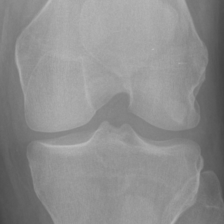
\includegraphics[width=2cm]{figs/KL0-sample.png} \\
        \hline
        1 (duvidoso) & 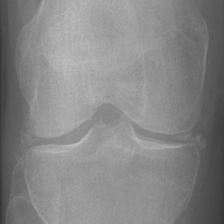
\includegraphics[width=2cm]{figs/KL1-sample.png} \\
        \hline
        2 (mínimo) & 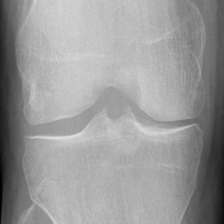
\includegraphics[width=2cm]{figs/KL2-sample.png} \\
        \hline
        3 (moderado) & 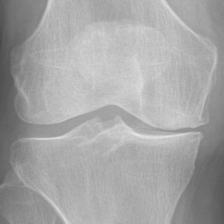
\includegraphics[width=2cm]{figs/KL3-sample.png} \\
        \hline
        4 (severo) & 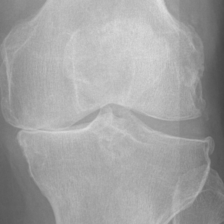
\includegraphics[width=2cm]{figs/KL4-sample.png} \\
        \hline
    \end{tabular}
    \caption{Escala de Kellgren/Lawrence para classificação da severidade de osteoartrite.}
    \label{tabela-kl}
\end{table}

\section{Visão Computacional na Saúde}\label{sec:visao-computacional}

A visão computacional é uma subárea da inteligência artificial (IA) que tem como objetivo automatizar a análise de imagens digitais, permitindo que a máquina "veja" e interprete o conteúdo visual de uma imagem. Essa ideia emergiu por volta da década de 1960, quando pioneiros como David Marr e Hans Moravec se questionaram da possibilidade de tornar computadores capazes de enxergar. Desde então, com o desenvolvimento de pesquisas na área de IA e melhorias em hardware, houveram diversos avanços na área, como o surgimento de algoritmos para detecção de bordas, detecção de objetos, segmentação de imagens, entre outros \cite{huggingface2024}.

Na área da saúde, a visão computacional tem sido muito utilizada para melhorar a acurácia de diagnósticos, automatização de tarefas clínicas e tratamentos médicos. Ao analisar imagens médicas, como radiografias, tomografias, ressonâncias magnéticas e ultrassonografias, a máquina pode detectar e classificar patologias com maior precisão e rapidez do que um médico humano. Além disso, a visão computacional pode ser utilizada para monitorar o progresso de doenças, monitorar a eficácia de tratamentos e até mesmo recomendar tratamentos personalizados para pacientes \cite{JAVAID2024792}.

\section{Aprendizado Profundo}\label{sec:aprendizado-profundo}

O uso de modelos de aprendizado profundo baseados em redes neurais convolucionais (RNCs) tem ganhado espaço em tarefas de visão computacional. Aprendizado por transferência também é amplamente utilizado para reduzir o uso de recursos computacionais para tarefas que já são executadas por modelos existentes, como as redes residuais (ResNet), Visual Geometry Group (VGG) e as redes densamente conectadas (DenseNet) \cite{Tariq2023}. Enquanto o uso de RNCs tem se mostrado útil em soluções de detecção em imagens médicas, a operação de convolução limita o relacionamento entre pixels distantes numa imagem. Para tanto, a habilidade de codificar dependências de longo alcance tem sido possível graças às arquiteturas de aprendizado profundas baseadas em atenção, como o Vision Transformer (ViT). Tais modelos de ViT têm sido empregados para várias tarefas, incluindo classificação e detecção de objetos \cite{Shamshad2023}.

% \section{Transferência de Aprendizado e Ajuste Fino}\label{sec:ajuste-fino}